% !TeX root = Thesis.tex

\newpage 
\section*{Result Diagrams}

\subsection*{Linear Program}
\begin{figure}[!htbp]
\centering
\begin{tikzpicture}[level distance=1cm,
  level 1/.style={sibling distance=9cm},
  level 2/.style={sibling distance=5cm}]
  \node {n=3}
    child { node {$H$ exists}
      child { node {$\underset{\raisebox{-0.8em}{3}}{\text{LP integral solution}}$} }
      child { node {$\underset{\raisebox{-0.8em}{0}}{\text{LP fractional solution}}$} }
    }
    child { node {$H$ does not exist}
      child { node {$\underset{\raisebox{-0.8em}{1}}{\text{LP infeasible}}$} }
      child { node {$\underset{\raisebox{-0.8em}{0}}{\text{LP fractional solution}}$} }
    };
\end{tikzpicture}

\begin{tikzpicture}[level distance=1cm,
  level 1/.style={sibling distance=9cm},
  level 2/.style={sibling distance=5cm}]
  \node {n=4}
    child { node {$H$ exists}
      child { node {$\underset{\raisebox{-0.8em}{6}}{\text{LP integral solution}}$} }
      child { node {$\underset{\raisebox{-0.8em}{0}}{\text{LP fractional solution}}$} }
    }
    child { node {$H$ does not exist}
      child { node {$\underset{\raisebox{-0.8em}{5}}{\text{LP infeasible}}$} }
      child { node {$\underset{\raisebox{-0.8em}{0}}{\text{LP fractional solution}}$} }
    };
\end{tikzpicture}

\begin{tikzpicture}[level distance=1cm,
  level 1/.style={sibling distance=9cm},
  level 2/.style={sibling distance=5cm}]
  \node {n=5}
    child { node {$H$ exists}
      child { node {$\underset{\raisebox{-0.8em}{10}}{\text{LP integral solution}}$} }
      child { node {$\underset{\raisebox{-0.8em}{1}}{\text{LP fractional solution}}$} }
    }
    child { node {$H$ does not exist}
      child { node {$\underset{\raisebox{-0.8em}{20}}{\text{LP infeasible}}$} }
      child { node {$\underset{\raisebox{-0.8em}{3}}{\text{LP fractional solution}}$} }
    };
\end{tikzpicture}

\begin{tikzpicture}[level distance=1cm,
  level 1/.style={sibling distance=9cm},
  level 2/.style={sibling distance=5cm}]
  \node {n=6}
    child { node {$H$ exists}
      child { node {$\underset{\raisebox{-0.8em}{17}}{\text{LP integral solution}}$} }
      child { node {$\underset{\raisebox{-0.8em}{11}}{\text{LP fractional solution}}$} }
    }
    child { node {$H$ does not exist}
      child { node {$\underset{\raisebox{-0.8em}{107}}{\text{LP infeasible}}$} }
      child { node {$\underset{\raisebox{-0.8em}{21}}{\text{LP fractional solution}}$} }
    };
\end{tikzpicture}

\begin{tikzpicture}[level distance=1cm,
  level 1/.style={sibling distance=9cm},
  level 2/.style={sibling distance=5cm}]
  \node {n=7}
    child { node {$H$ exists}
      child { node {$\underset{\raisebox{-0.8em}{29}}{\text{LP integral solution}}$} }
      child { node {$\underset{\raisebox{-0.8em}{48}}{\text{LP fractional solution}}$} }
    }
    child { node {$H$ does not exist}
      child { node {$\underset{\raisebox{-0.8em}{767}}{\text{LP infeasible}}$} }
      child { node {$\underset{\raisebox{-0.8em}{200}}{\text{LP fractional solution}}$} }
    };
\end{tikzpicture}

\begin{tikzpicture}[level distance=1cm,
  level 1/.style={sibling distance=9cm},
  level 2/.style={sibling distance=5cm}]
  \node {n=8}
    child { node {$H$ exists}
      child { node {$\underset{\raisebox{-0.8em}{51}}{\text{LP integral solution}}$} }
      child { node {$\underset{\raisebox{-0.8em}{256}}{\text{LP fractional solution}}$} }
    }
    child { node {$H$ does not exist}
      child { node {$\underset{\raisebox{-0.8em}{9380}}{\text{LP infeasible}}$} }
      child { node {$\underset{\raisebox{-0.8em}{2659}}{\text{LP fractional solution}}$} }
    };
\end{tikzpicture}

\caption{LP outcomes for different values of $n$ on base linear program.} 
\footnotemark 
\label{fig::linear_program_diagram} 
\end{figure}

\footnotetext{
The total number of simple graphs on $n=2,3,4,\dots$ unlabeled nodes is the sequence $2, 4, 11, 34, 156, 1044, 12346, \dots$ given by \href{https://oeis.org/A000088}{\texttt{A000088}}. \\
The IP integral solution sequence $2, 3, 6, 10, 17, 29, 51, \dots$ is given by \href{https://oeis.org/A285665}{A285665}. \\
The total number of graphs which are squares is the sequence $2, 3, 6, 11, 28, 77, 307, \dots$ given by \href{https://oeis.org/A382181}{A382181}.}

\newpage

\subsubsection*{Max Objective Function}

\begin{figure}[!htbp]
\centering
\begin{tikzpicture}[level distance=1cm,
  level 1/.style={sibling distance=9cm},
  level 2/.style={sibling distance=5cm}]
  \node {n=3}
    child { node {$H$ exists}
      child { node {$\underset{\raisebox{-0.8em}{3}}{\text{LP integral solution}}$} }
      child { node {$\underset{\raisebox{-0.8em}{0}}{\text{LP fractional solution}}$} }
    }
    child { node {$H$ does not exist}
      child { node {$\underset{\raisebox{-0.8em}{1}}{\text{LP infeasible}}$} }
      child { node {$\underset{\raisebox{-0.8em}{0}}{\text{LP fractional solution}}$} }
    };
\end{tikzpicture}

\begin{tikzpicture}[level distance=1cm,
  level 1/.style={sibling distance=9cm},
  level 2/.style={sibling distance=5cm}]
  \node {n=4}
    child { node {$H$ exists}
      child { node {$\underset{\raisebox{-0.8em}{6}}{\text{LP integral solution}}$} }
      child { node {$\underset{\raisebox{-0.8em}{0}}{\text{LP fractional solution}}$} }
    }
    child { node {$H$ does not exist}
      child { node {$\underset{\raisebox{-0.8em}{5}}{\text{LP infeasible}}$} }
      child { node {$\underset{\raisebox{-0.8em}{0}}{\text{LP fractional solution}}$} }
    };
\end{tikzpicture}

\begin{tikzpicture}[level distance=1cm,
  level 1/.style={sibling distance=9cm},
  level 2/.style={sibling distance=5cm}]
  \node {n=5}
    child { node {$H$ exists}
      child { node {$\underset{\raisebox{-0.8em}{11}}{\text{LP integral solution}}$} }
      child { node {$\underset{\raisebox{-0.8em}{0}}{\text{LP fractional solution}}$} }
    }
    child { node {$H$ does not exist}
      child { node {$\underset{\raisebox{-0.8em}{20}}{\text{LP infeasible}}$} }
      child { node {$\underset{\raisebox{-0.8em}{3}}{\text{LP fractional solution}}$} }
    };
\end{tikzpicture}

\begin{tikzpicture}[level distance=1cm,
  level 1/.style={sibling distance=9cm},
  level 2/.style={sibling distance=5cm}]
  \node {n=6}
    child { node {$H$ exists}
      child { node {$\underset{\raisebox{-0.8em}{24}}{\text{LP integral solution}}$} }
      child { node {$\underset{\raisebox{-0.8em}{4}}{\text{LP fractional solution}}$} }
    }
    child { node {$H$ does not exist}
      child { node {$\underset{\raisebox{-0.8em}{107}}{\text{LP infeasible}}$} }
      child { node {$\underset{\raisebox{-0.8em}{21}}{\text{LP fractional solution}}$} }
    };
\end{tikzpicture}

\begin{tikzpicture}[level distance=1cm,
  level 1/.style={sibling distance=9cm},
  level 2/.style={sibling distance=5cm}]
  \node {n=7}
    child { node {$H$ exists}
      child { node {$\underset{\raisebox{-0.8em}{43}}{\text{LP integral solution}}$} }
      child { node {$\underset{\raisebox{-0.8em}{34}}{\text{LP fractional solution}}$} }
    }
    child { node {$H$ does not exist}
      child { node {$\underset{\raisebox{-0.8em}{767}}{\text{LP infeasible}}$} }
      child { node {$\underset{\raisebox{-0.8em}{200}}{\text{LP fractional solution}}$} }
    };
\end{tikzpicture}

\begin{tikzpicture}[level distance=1cm,
  level 1/.style={sibling distance=9cm},
  level 2/.style={sibling distance=5cm}]
  \node {n=8}
    child { node {$H$ exists}
      child { node {$\underset{\raisebox{-0.8em}{102}}{\text{LP integral solution}}$} }
      child { node {$\underset{\raisebox{-0.8em}{205}}{\text{LP fractional solution}}$} }
    }
    child { node {$H$ does not exist}
      child { node {$\underset{\raisebox{-0.8em}{9380}}{\text{LP infeasible}}$} }
      child { node {$\underset{\raisebox{-0.8em}{2659}}{\text{LP fractional solution}}$} }
    };
\end{tikzpicture}

\caption{LP outcomes for different values of $n$ on the linear program with max objective function.}
\footnotemark
\label{fig::max_objective_function_diagram}
\end{figure}

\footnotetext{The LP integer 
solution sequence $3, 6, 11, 22, 42, 102, \dots$ is very similar to the 
number of distinct characteristic polynomials of tress with $n$ nodes - \href{https://oeis.org/A226594}{A226594}.}

\newpage

\subsubsection*{Min Objective Function}

\begin{figure}[!htbp]
\centering
\begin{tikzpicture}[level distance=1cm,
  level 1/.style={sibling distance=9cm},
  level 2/.style={sibling distance=5cm}]
  \node {n=3}
    child { node {$H$ exists}
      child { node {$\underset{\raisebox{-0.8em}{2}}{\text{LP integral solution}}$} }
      child { node {$\underset{\raisebox{-0.8em}{1}}{\text{LP fractional solution}}$} }
    }
    child { node {$H$ does not exist}
      child { node {$\underset{\raisebox{-0.8em}{1}}{\text{LP infeasible}}$} }
      child { node {$\underset{\raisebox{-0.8em}{0}}{\text{LP fractional solution}}$} }
    };
\end{tikzpicture}

\begin{tikzpicture}[level distance=1cm,
  level 1/.style={sibling distance=9cm},
  level 2/.style={sibling distance=5cm}]
  \node {n=4}
    child { node {$H$ exists}
      child { node {$\underset{\raisebox{-0.8em}{3}}{\text{LP integral solution}}$} }
      child { node {$\underset{\raisebox{-0.8em}{3}}{\text{LP fractional solution}}$} }
    }
    child { node {$H$ does not exist}
      child { node {$\underset{\raisebox{-0.8em}{5}}{\text{LP infeasible}}$} }
      child { node {$\underset{\raisebox{-0.8em}{0}}{\text{LP fractional solution}}$} }
    };
\end{tikzpicture}

\begin{tikzpicture}[level distance=1cm,
  level 1/.style={sibling distance=9cm},
  level 2/.style={sibling distance=5cm}]
  \node {n=5}
    child { node {$H$ exists}
      child { node {$\underset{\raisebox{-0.8em}{3}}{\text{LP integral solution}}$} }
      child { node {$\underset{\raisebox{-0.8em}{8}}{\text{LP fractional solution}}$} }
    }
    child { node {$H$ does not exist}
      child { node {$\underset{\raisebox{-0.8em}{20}}{\text{LP infeasible}}$} }
      child { node {$\underset{\raisebox{-0.8em}{3}}{\text{LP fractional solution}}$} }
    };
\end{tikzpicture}

\begin{tikzpicture}[level distance=1cm,
  level 1/.style={sibling distance=9cm},
  level 2/.style={sibling distance=5cm}]
  \node {n=6}
    child { node {$H$ exists}
      child { node {$\underset{\raisebox{-0.8em}{4}}{\text{LP integral solution}}$} }
      child { node {$\underset{\raisebox{-0.8em}{24}}{\text{LP fractional solution}}$} }
    }
    child { node {$H$ does not exist}
      child { node {$\underset{\raisebox{-0.8em}{107}}{\text{LP infeasible}}$} }
      child { node {$\underset{\raisebox{-0.8em}{21}}{\text{LP fractional solution}}$} }
    };
\end{tikzpicture}

\begin{tikzpicture}[level distance=1cm,
  level 1/.style={sibling distance=9cm},
  level 2/.style={sibling distance=5cm}]
  \node {n=7}
    child { node {$H$ exists}
      child { node {$\underset{\raisebox{-0.8em}{5}}{\text{LP integral solution}}$} }
      child { node {$\underset{\raisebox{-0.8em}{72}}{\text{LP fractional solution}}$} }
    }
    child { node {$H$ does not exist}
      child { node {$\underset{\raisebox{-0.8em}{767}}{\text{LP infeasible}}$} }
      child { node {$\underset{\raisebox{-0.8em}{200}}{\text{LP fractional solution}}$} }
    };
\end{tikzpicture}

\caption{LP outcomes for different values of $n$ on the linear program with min objective function.}
\footnotemark
\label{fig::min_objective_function_diagram}
\end{figure}

\newpage

\subsubsection*{Single Triangular Decomposition}
\begin{figure}[!htbp]
\centering

\begin{tikzpicture}[level distance=1cm,
  level 1/.style={sibling distance=9cm},
  level 2/.style={sibling distance=5cm}]
  \node {n=4}
    child { node {$H$ exists}
      child { node {$\underset{\raisebox{-0.8em}{6}}{\text{LP integral solution}}$} }
      child { node {$\underset{\raisebox{-0.8em}{0}}{\text{LP fractional solution}}$} }
    }
    child { node {$H$ does not exist}
      child { node {$\underset{\raisebox{-0.8em}{5}}{\text{LP infeasible}}$} }
      child { node {$\underset{\raisebox{-0.8em}{0}}{\text{LP fractional solution}}$} }
    };
\end{tikzpicture}

\begin{tikzpicture}[level distance=1cm,
  level 1/.style={sibling distance=9cm},
  level 2/.style={sibling distance=5cm}]
  \node {n=5}
    child { node {$H$ exists}
      child { node {$\underset{\raisebox{-0.8em}{11}}{\text{LP integral solution}}$} }
      child { node {$\underset{\raisebox{-0.8em}{0}}{\text{LP fractional solution}}$} }
    }
    child { node {$H$ does not exist}
      child { node {$\underset{\raisebox{-0.8em}{20}}{\text{LP infeasible}}$} }
      child { node {$\underset{\raisebox{-0.8em}{3}}{\text{LP fractional solution}}$} }
    };
\end{tikzpicture}

\begin{tikzpicture}[level distance=1cm,
  level 1/.style={sibling distance=9cm},
  level 2/.style={sibling distance=5cm}]
  \node {n=6}
    child { node {$H$ exists}
      child { node {$\underset{\raisebox{-0.8em}{24}}{\text{LP integral solution}}$} }
      child { node {$\underset{\raisebox{-0.8em}{4}}{\text{LP fractional solution}}$} }
    }
    child { node {$H$ does not exist}
      child { node {$\underset{\raisebox{-0.8em}{111}}{\text{LP infeasible}}$} }
      child { node {$\underset{\raisebox{-0.8em}{17}}{\text{LP fractional solution}}$} }
    };
\end{tikzpicture}

\begin{tikzpicture}[level distance=1cm,
  level 1/.style={sibling distance=9cm},
  level 2/.style={sibling distance=5cm}]
  \node {n=7}
    child { node {$H$ exists}
      child { node {$\underset{\raisebox{-0.8em}{51}}{\text{LP integral solution}}$} }
      child { node {$\underset{\raisebox{-0.8em}{26}}{\text{LP fractional solution}}$} }
    }
    child { node {$H$ does not exist}
      child { node {$\underset{\raisebox{-0.8em}{831}}{\text{LP infeasible}}$} }
      child { node {$\underset{\raisebox{-0.8em}{136}}{\text{LP fractional solution}}$} }
    };
\end{tikzpicture}

\begin{tikzpicture}[level distance=1cm,
  level 1/.style={sibling distance=9cm},
  level 2/.style={sibling distance=5cm}]
  \node {n=8}
    child { node {$H$ exists}
      child { node {$\underset{\raisebox{-0.8em}{142}}{\text{LP integral solution}}$} }
      child { node {$\underset{\raisebox{-0.8em}{165}}{\text{LP fractional solution}}$} }
    }
    child { node {$H$ does not exist}
      child { node {$\underset{\raisebox{-0.8em}{10351}}{\text{LP infeasible}}$} }
      child { node {$\underset{\raisebox{-0.8em}{1688}}{\text{LP fractional solution}}$} }
    };
\end{tikzpicture}

\caption{LP outcomes for different values of $n$ on the linear program with max objective function 
and single triangular decomposition.}
\label{fig::single_triangular_decomposition_diagram}
\end{figure}

\newpage

\begin{figure}[!htbp]
\centering

\begin{tikzpicture}[level distance=1cm,
  level 1/.style={sibling distance=9cm},
  level 2/.style={sibling distance=5cm}]
  \node {n=4}
    child { node {$H$ exists}
      child { node {$\underset{\raisebox{-0.8em}{6}}{\text{LP integral solution}}$} }
      child { node {$\underset{\raisebox{-0.8em}{0}}{\text{LP fractional solution}}$} }
    }
    child { node {$H$ does not exist}
      child { node {$\underset{\raisebox{-0.8em}{5}}{\text{LP infeasible}}$} }
      child { node {$\underset{\raisebox{-0.8em}{0}}{\text{LP fractional solution}}$} }
    };
\end{tikzpicture}

\begin{tikzpicture}[level distance=1cm,
  level 1/.style={sibling distance=9cm},
  level 2/.style={sibling distance=5cm}]
  \node {n=5}
    child { node {$H$ exists}
      child { node {$\underset{\raisebox{-0.8em}{11}}{\text{LP integral solution}}$} }
      child { node {$\underset{\raisebox{-0.8em}{0}}{\text{LP fractional solution}}$} }
    }
    child { node {$H$ does not exist}
      child { node {$\underset{\raisebox{-0.8em}{21}}{\text{LP infeasible}}$} }
      child { node {$\underset{\raisebox{-0.8em}{2}}{\text{LP fractional solution}}$} }
    };
\end{tikzpicture}

\begin{tikzpicture}[level distance=1cm,
  level 1/.style={sibling distance=9cm},
  level 2/.style={sibling distance=5cm}]
  \node {n=6}
    child { node {$H$ exists}
      child { node {$\underset{\raisebox{-0.8em}{22}}{\text{LP integral solution}}$} }
      child { node {$\underset{\raisebox{-0.8em}{6}}{\text{LP fractional solution}}$} }
    }
    child { node {$H$ does not exist}
      child { node {$\underset{\raisebox{-0.8em}{119}}{\text{LP infeasible}}$} }
      child { node {$\underset{\raisebox{-0.8em}{9}}{\text{LP fractional solution}}$} }
    };
\end{tikzpicture}

\begin{tikzpicture}[level distance=1cm,
  level 1/.style={sibling distance=9cm},
  level 2/.style={sibling distance=5cm}]
  \node {n=7}
    child { node {$H$ exists}
      child { node {$\underset{\raisebox{-0.8em}{51}}{\text{LP integral solution}}$} }
      child { node {$\underset{\raisebox{-0.8em}{26}}{\text{LP fractional solution}}$} }
    }
    child { node {$H$ does not exist}
      child { node {$\underset{\raisebox{-0.8em}{877}}{\text{LP infeasible}}$} }
      child { node {$\underset{\raisebox{-0.8em}{90}}{\text{LP fractional solution}}$} }
    };
\end{tikzpicture}

\begin{tikzpicture}[level distance=1cm,
  level 1/.style={sibling distance=9cm},
  level 2/.style={sibling distance=5cm}]
  \node {n=8}
    child { node {$H$ exists}
      child { node {$\underset{\raisebox{-0.8em}{142}}{\text{LP integral solution}}$} }
      child { node {$\underset{\raisebox{-0.8em}{165}}{\text{LP fractional solution}}$} }
    }
    child { node {$H$ does not exist}
      child { node {$\underset{\raisebox{-0.8em}{10708}}{\text{LP infeasible}}$} }
      child { node {$\underset{\raisebox{-0.8em}{1331}}{\text{LP fractional solution}}$} }
    };
\end{tikzpicture}

\caption{LP outcomes for different values of $n$ on the linear program with max objective function 
and single triangular decomposition with recursion for tie-breaking.}
\label{fig::recursive_single_triangular_decomposition_diagram}
\end{figure}

\newpage

\subsubsection*{Rounding}

\begin{figure}[!htbp]
\centering

\begin{tikzpicture}[level distance=1.25cm,
  level 1/.style={sibling distance=8cm},
  level 2/.style={sibling distance=4cm},
  level 3/.style={sibling distance=3cm}]
  \node {n=5}
    child { node {$H$ exists}
      child { node {$\underset{\raisebox{-0.8em}{11}}{\text{LP integer}}$} }
      child { node {$\underset{\raisebox{-0.8em}{0}}{\text{LP fractional}}$} 
        child { node {$\underset{\raisebox{-0.8em}{0}}{\text{Rounding}}$}  }
        child { node {$\underset{\raisebox{-0.8em}{0}}{\text{Infeasible}}$}  }
      }
    }
    child { node {$H$ does not exist}
      child { node {$\underset{\raisebox{-0.8em}{20}}{\text{LP infeasible}}$} }
      child { node {$\underset{\raisebox{-0.8em}{3}}{\text{LP fractional}}$} 
        child { node {$\underset{\raisebox{-0.8em}{0}}{\text{Rounding}}$}  }
        child { node {$\underset{\raisebox{-0.8em}{3}}{\text{Infeasible}}$}  }
      }
    };
\end{tikzpicture}

\begin{tikzpicture}[level distance=1.25cm,
  level 1/.style={sibling distance=8cm},
  level 2/.style={sibling distance=4cm},
  level 3/.style={sibling distance=3cm}]
  \node {n=6}
    child { node {$H$ exists}
      child { node {$\underset{\raisebox{-0.8em}{22}}{\text{LP integer}}$} }
      child { node {$\underset{\raisebox{-0.8em}{6}}{\text{LP fractional}}$} 
        child { node {$\underset{\raisebox{-0.8em}{6}}{\text{Rounding}}$}  }
        child { node {$\underset{\raisebox{-0.8em}{0}}{\text{Infeasible}}$}  }
      }
    }
    child { node {$H$ does not exist}
      child { node {$\underset{\raisebox{-0.8em}{107}}{\text{LP infeasible}}$} }
      child { node {$\underset{\raisebox{-0.8em}{21}}{\text{LP fractional}}$} 
        child { node {$\underset{\raisebox{-0.8em}{0}}{\text{Rounding}}$}  }
        child { node {$\underset{\raisebox{-0.8em}{21}}{\text{Infeasible}}$}  }
      }
    };
\end{tikzpicture}

\begin{tikzpicture}[level distance=1.25cm,
  level 1/.style={sibling distance=8cm},
  level 2/.style={sibling distance=4cm},
  level 3/.style={sibling distance=3cm}]
  \node {n=7}
    child { node {$H$ exists}
      child { node {$\underset{\raisebox{-0.8em}{43}}{\text{LP integer}}$} }
      child { node {$\underset{\raisebox{-0.8em}{34}}{\text{LP fractional}}$} 
        child { node {$\underset{\raisebox{-0.8em}{30}}{\text{Rounding}}$}  }
        child { node {$\underset{\raisebox{-0.8em}{4}}{\text{Infeasible}}$}  }
      }
    }
    child { node {$H$ does not exist}
      child { node {$\underset{\raisebox{-0.8em}{767}}{\text{LP infeasible}}$} }
      child { node {$\underset{\raisebox{-0.8em}{200}}{\text{LP fractional}}$} 
        child { node {$\underset{\raisebox{-0.8em}{0}}{\text{Rounding}}$}  }
        child { node {$\underset{\raisebox{-0.8em}{2000}}{\text{Infeasible}}$}  }
      }
    };
\end{tikzpicture}

\begin{tikzpicture}[level distance=1.25cm,
  level 1/.style={sibling distance=8cm},
  level 2/.style={sibling distance=4cm},
  level 3/.style={sibling distance=3cm}]
  \node {n=8}
    child { node {$H$ exists}
      child { node {$\underset{\raisebox{-0.8em}{102}}{\text{LP integer}}$} }
      child { node {$\underset{\raisebox{-0.8em}{205}}{\text{LP fractional}}$} 
        child { node {$\underset{\raisebox{-0.8em}{144}}{\text{Rounding}}$}  }
        child { node {$\underset{\raisebox{-0.8em}{61}}{\text{Infeasible}}$}  }
      }
    }
    child { node {$H$ does not exist}
      child { node {$\underset{\raisebox{-0.8em}{9380}}{\text{LP infeasible}}$} }
      child { node {$\underset{\raisebox{-0.8em}{2659}}{\text{LP fractional}}$} 
        child { node {$\underset{\raisebox{-0.8em}{0}}{\text{Rounding}}$}  }
        child { node {$\underset{\raisebox{-0.8em}{2659}}{\text{Infeasible}}$}  }
      }
    };
\end{tikzpicture}

\caption{LP outcomes for different values of $n$ on the linear program with max objective function 
and using rounding for fractional solutions.}
\label{fig::rounding_max_objective_function_diagram}
\end{figure}

\newpage

\begin{figure}[!htbp]
\centering

\begin{tikzpicture}[level distance=1.25cm,
  level 1/.style={sibling distance=8cm},
  level 2/.style={sibling distance=4cm},
  level 3/.style={sibling distance=3cm}]
  \node {n=5}
    child { node {$H$ exists}
      child { node {$\underset{\raisebox{-0.8em}{11}}{\text{LP integer}}$} }
      child { node {$\underset{\raisebox{-0.8em}{0}}{\text{LP fractional}}$} 
        child { node {$\underset{\raisebox{-0.8em}{0}}{\text{Rounding}}$}  }
        child { node {$\underset{\raisebox{-0.8em}{0}}{\text{Infeasible}}$}  }
      }
    }
    child { node {$H$ does not exist}
      child { node {$\underset{\raisebox{-0.8em}{20}}{\text{LP infeasible}}$} }
      child { node {$\underset{\raisebox{-0.8em}{3}}{\text{LP fractional}}$} 
        child { node {$\underset{\raisebox{-0.8em}{0}}{\text{Rounding}}$}  }
        child { node {$\underset{\raisebox{-0.8em}{3}}{\text{Infeasible}}$}  }
      }
    };
\end{tikzpicture}

\begin{tikzpicture}[level distance=1.25cm,
  level 1/.style={sibling distance=8cm},
  level 2/.style={sibling distance=4cm},
  level 3/.style={sibling distance=3cm}]
  \node {n=6}
    child { node {$H$ exists}
      child { node {$\underset{\raisebox{-0.8em}{22}}{\text{LP integer}}$} }
      child { node {$\underset{\raisebox{-0.8em}{6}}{\text{LP fractional}}$} 
        child { node {$\underset{\raisebox{-0.8em}{6}}{\text{Rounding}}$}  }
        child { node {$\underset{\raisebox{-0.8em}{0}}{\text{Infeasible}}$}  }
      }
    }
    child { node {$H$ does not exist}
      child { node {$\underset{\raisebox{-0.8em}{111}}{\text{LP infeasible}}$} }
      child { node {$\underset{\raisebox{-0.8em}{17}}{\text{LP fractional}}$} 
        child { node {$\underset{\raisebox{-0.8em}{0}}{\text{Rounding}}$}  }
        child { node {$\underset{\raisebox{-0.8em}{17}}{\text{Infeasible}}$}  }
      }
    };
\end{tikzpicture}

\begin{tikzpicture}[level distance=1.25cm,
  level 1/.style={sibling distance=8cm},
  level 2/.style={sibling distance=4cm},
  level 3/.style={sibling distance=3cm}]
  \node {n=7}
    child { node {$H$ exists}
      child { node {$\underset{\raisebox{-0.8em}{51}}{\text{LP integer}}$} }
      child { node {$\underset{\raisebox{-0.8em}{26}}{\text{LP fractional}}$} 
        child { node {$\underset{\raisebox{-0.8em}{24}}{\text{Rounding}}$}  }
        child { node {$\underset{\raisebox{-0.8em}{2}}{\text{Infeasible}}$}  }
      }
    }
    child { node {$H$ does not exist}
      child { node {$\underset{\raisebox{-0.8em}{831}}{\text{LP infeasible}}$} }
      child { node {$\underset{\raisebox{-0.8em}{136}}{\text{LP fractional}}$} 
        child { node {$\underset{\raisebox{-0.8em}{0}}{\text{Rounding}}$}  }
        child { node {$\underset{\raisebox{-0.8em}{136}}{\text{Infeasible}}$}  }
      }
    };
\end{tikzpicture}

\begin{tikzpicture}[level distance=1.25cm,
  level 1/.style={sibling distance=8cm},
  level 2/.style={sibling distance=4cm},
  level 3/.style={sibling distance=3cm}]
  \node {n=8}
    child { node {$H$ exists}
      child { node {$\underset{\raisebox{-0.8em}{142}}{\text{LP integer}}$} }
      child { node {$\underset{\raisebox{-0.8em}{165}}{\text{LP fractional}}$} 
        child { node {$\underset{\raisebox{-0.8em}{121}}{\text{Rounding}}$}  }
        child { node {$\underset{\raisebox{-0.8em}{44}}{\text{Infeasible}}$}  }
      }
    }
    child { node {$H$ does not exist}
      child { node {$\underset{\raisebox{-0.8em}{9380}}{\text{LP infeasible}}$} }
      child { node {$\underset{\raisebox{-0.8em}{2659}}{\text{LP fractional}}$} 
        child { node {$\underset{\raisebox{-0.8em}{0}}{\text{Rounding}}$}  }
        child { node {$\underset{\raisebox{-0.8em}{2659}}{\text{Infeasible}}$}  }
      }
    };
\end{tikzpicture}

\caption{LP outcomes for different values of $n$ on the linear program with max objective function, single 
triangular decomposition and using rounding for fractional solutions.}
\label{fig::rounding_triangular_max_objective_function_diagram}
\end{figure}

\newpage

\subsection*{Dual Program}

\begin{figure}[!htbp]
\centering

\begin{tikzpicture}[
  level distance=1.25cm,
  level 1/.style={sibling distance=9cm},
  level 2/.style={sibling distance=4.1cm},
  level 3/.style={sibling distance=2.1cm},
  every node/.style={align=center, font=\tiny}
]

\node {n = 6}
  child { node {$H$ exists}
    child { node {$\underset{\raisebox{-0.8em}{}}{\text{Primal integer}}$} 
      child { node {$\underset{\raisebox{-0.8em}{}}{\text{Dual feasible}}$}  }
      child { node {$\underset{\raisebox{-0.8em}{}}{\text{Dual infeasible}}$}  }
    }
    child { node {$\underset{\raisebox{-0.8em}{}}{\text{Primal fractional}}$} 
      child { node {$\underset{\raisebox{-0.8em}{}}{\text{Dual feasible}}$}  }
      child { node {$\underset{\raisebox{-0.8em}{}}{\text{Dual unbounded}}$}  }
    }
  }
  child { node {$H$ does not exist}
    child { node {$\underset{\raisebox{-0.8em}{}}{\text{Primal infeasible}}$} 
      child { node {$\underset{\raisebox{-0.8em}{}}{\text{Dual feasible }}$}  }
      child { node {$\underset{\raisebox{-0.8em}{}}{\text{Dual infeasible}}$}  }
    }
    child { node {$\underset{\raisebox{-0.8em}{}}{\text{Primal fractional}}$} 
      child { node {$\underset{\raisebox{-0.8em}{}}{\text{Dual feasible }}$}  }
      child { node {$\underset{\raisebox{-0.8em}{}}{\text{Dual infeasible}}$}  }
    }
  };

\end{tikzpicture}

\caption{LP outcomes for different values of $n$ on the dual linear program.}
\label{fig::duak_objective_function_diagram}
\end{figure}

\newpage